\documentclass{article}

\begin{document}

\section{Work Environment}

\subsection{Force Yourself to Use the Command Line}

I would highly suggest that you force yourself to use the Linux command line terminal and avoid using the file explorer GUI as much as possible. It will be initially painful but massively beneficial, and if you learn to type fast (which you should), then using the terminal will very often be significantly faster than using a GUI. Even if this were not true, there are simply many tasks that cannot be done without a command line. (As stated in \textit{The Pragmatic Programmer} by Hunt and Thomas, ``A benefit of GUIs is WYSIWYG -- what you see is what you get. The disadvantage is WYSIAYG -- what you see is \textit{all} you get.'') In all three programming jobs that I have ever had, I had to be competent with the Linux command line.

\subsection{Editor}

I am not as enthusiastic about Vim (the \lstinline{vi} command) as other instructors are. I do think everyone should learn Vim because, as a fast typer, I often find that in certain situations (e.g. when I need to make quick modifications to a file), it is faster to use Vim than to switch windows to a more flashy editor such as Sublime Text. That said, you should figure out which editor works best for you. I personally most prefer Sublime Text, Atom, and Notepad++. You can try an IDE (e.g. Visual Studio) as well, but once makefiles become required in the programming assignments in this class, using an IDE could get in the way. Moreover, differences in the IDE's compiler (e.g. Visual Studio's compiler) vs. \lstinline{gcc}, the compiler that the autograder will use, could lead to unexpected failures when you submit your code to the autograder, e.g. if Visual Studio's compiler permits you to do something in your code that \lstinline{gcc} does not permit.

\subsection{Reference Environment is Linux}

The reference environment is Linux (specifically Ubuntu 18.04, but I don't think that the specific Linux distribution matters). This is the environment in which the Gradescope autograder runs your code. Thus, you should ideally work in a Linux environment and make sure your code compiles in one. You should not use the Gradescope autograder as your compiler (that is, you should try to make sure the code works in your work environment before submitting to the autograder, instead of blindly submitting to the autograder after every single modification to your code), because the Gradescope autograder gives much less informative messages than the compiler does, and also because I won't be writing autograders for you in the real world. If you already have a Linux computer, then this should not be an issue.

Below, I talk about options for Mac/Windows users. I will say that I have only ever used Linux and Windows computers, so anything that I say about Mac computers is based on what I've heard from friends or previous students (from when I taught ECS 36A last spring).

\subsubsection{If You Have a Mac Computer}

If you have a Mac computer, your environment is close to a Linux environment as far as C programming is concerned, but it differs significantly in the following ways:

\begin{itemize}[itemsep=0mm, parsep=0pt]
\item As far as I'm aware, Mac computers do not have \lstinline{gdb}. \lstinline{gdb} is the only debugger that I will demonstrate during lecture. If you insist on using a Mac and not bothering to figure out how to use the CSIF, then I ask that you become comfortable with a debugger on the Mac, because if you ask for help during office hours, the TA may ask you to do certain things with a debugger as they try to help you, and if the TA is only familiar with \lstinline{gdb}, then you will need to know how to do what they're suggesting on a different debugger.
\item There are certain compiler warnings (which become compiler errors, since the autograder will use the \lstinline{-Werror} flag when it uses \lstinline{gcc} to compile your code) that can be generated by \lstinline{gcc} in a Linux environment but not by \lstinline{gcc} in a Mac environment. The one that comes to mind is the ``misleading indentation'' error message. Below is an example of this. If you are using a Mac and try to compile the code shown below, you should find that you get no compiler error message. (Be careful about copying the code directly from this document; any quotation marks in the code may become distored, and you'll have to retype them.)

\begin{lstlisting}
$ cat main.c 
#include <stdio.h>

int main()
{
    if (5 == 5)
        printf("Hi\n");
        printf("Bye\n");
}
$ gcc -Wall -Werror main.c 
main.c: In function 'main':
main.c:5:5: error: this 'if' clause does not guard... [-Werror=misleading-indentation]
     if (5 == 5)
     ^~
main.c:7:9: note: ...this statement, but the latter is misleadingly indented as if it were guarded by the 'if'
         printf("Bye\n");
         ^~~~~~
cc1: all warnings being treated as errors
$ 
\end{lstlisting}
\end{itemize}

Even if you use a Mac, \textbf{I most recommend that you use the CSIF}. I talk more about the CSIF below. Having never used a Mac, I don't know of alternatives, and I don't know how well dual booting works on a Mac either. You could try a virtual machine that runs a Linux environment. Depending on your computer's hardware, a virtual machine might be too demanding or run too slowly.

\textbf{Common error message}: When installing and trying to run the student VPN (PulseSecure), it seems that Mac users commonly encounter one or both of the following or something similar to these messages. (I can't remember if the second image was related or not.) I have been told by a friend of mine (who owns a Mac) that a way to deal with this is to go to System Preferences $\Rightarrow$ Security and Privacy $\Rightarrow$ General $\Rightarrow$ Allow your Mac to run PulseSecure. This seems to have worked for some students.\\

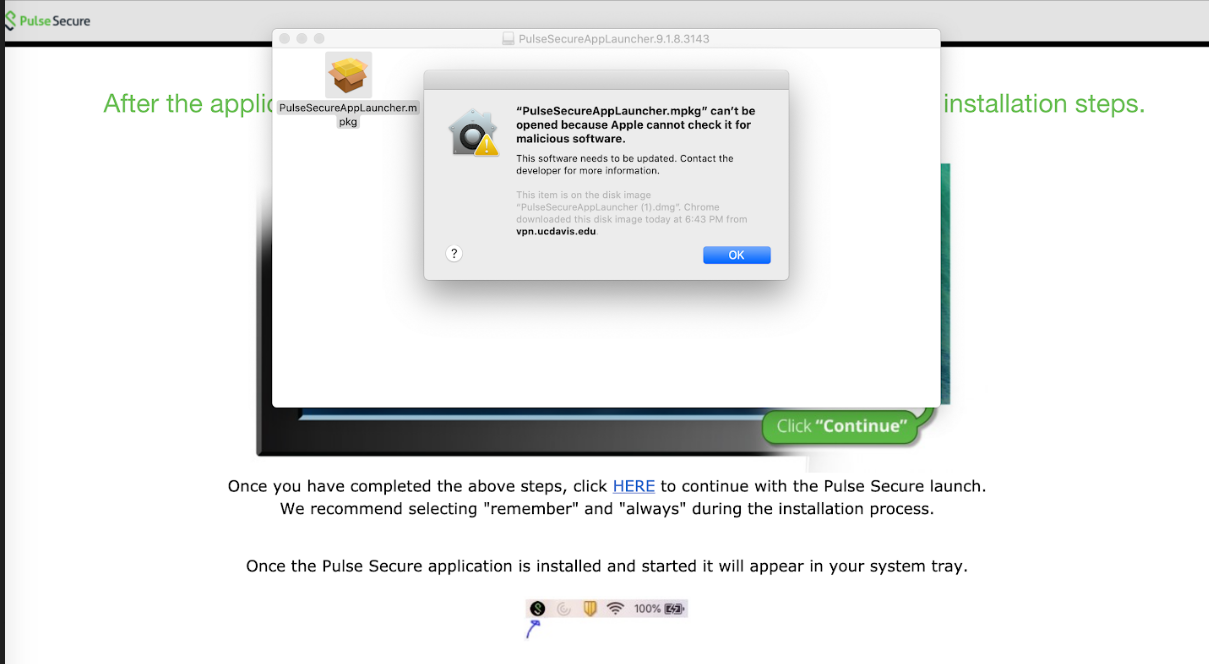
\includegraphics[scale=0.35]{mac_issue_1}

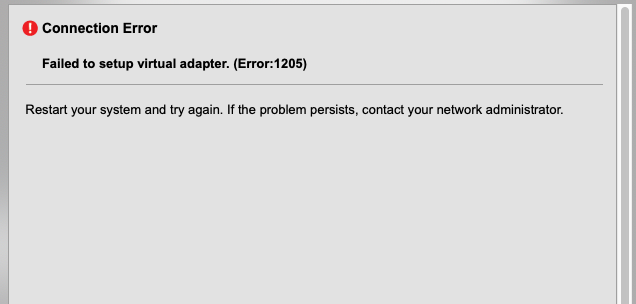
\includegraphics[scale=0.45]{mac_issue_2}

\subsubsection{If You Have a Windows Computer}

If you have a Windows computer, do note that the Windows command line significantly differs from the Linux command line; I recommend you use one of the below for a development environment if you are a Windows user. \textbf{I most recommend that you use the CSIF.} When I taught ECS 36A last spring, I did have students who used the Windows Subsystem for Linux and other similar options, and I never heard about any issues they had (whereas I did hear about issues from Mac users), but I don't know if that's because said Windows users ended up using the CSIF.

\begin{itemize}[itemsep=0mm, parsep=0pt]
\item CSIF. (I talk more about the CSIF below.)
    \begin{itemize}[itemsep=0mm, parsep=0pt]
    \item I believe the other options require a decent amount of setup. As someone who only owned a Windows laptop during his undergraduate career, I felt that the CSIF was the most convenient option whenever I needed a Linux environment. I personally did not have much luck with dual booting, but friends of mine had no issues with dual booting.
    \item You can use WinSCP or (more preferably) the Linux \lstinline{scp} command for transferring files.
    \end{itemize}
\item Virtual machine that runs a Linux environment.
    \begin{itemize}[itemsep=0mm, parsep=0pt]
    \item Depending on your computer, a virtual machine might be too demanding or run too slowly.
    \end{itemize}
\item Dual booting.
    \begin{itemize}[itemsep=0mm, parsep=0pt]
    \item Dual booting is when each time you turn on (or restart) your computer, you can choose which operating system (e.g. Windows or Linux) your computer loads.
    \item \textcolor{red}{Setting up dual booting renders your laptop unusable for a few hours.} Be aware of this in case you decide to configure dual booting in the middle of the quarter.
    \item As stated above, I never had much luck with dual booting, but friends of mine had no issues with it.
    \end{itemize}
\item Windows Subsystem for Linux.
\item Git Bash.
\item Moba XTerm.
\item Cygwin.
\end{itemize}

\subsubsection{CSIF}

In the basement of Kemper Hall, there are many computers that are known as the CSIF or the CSIF computers. I've no idea if you can physically access them during fall quarter, but that isn't necessary; you can instead log into a CSIF computer remotely.

\textbf{You must use a certain VPN when you log in to the CSIF.} Directions on this VPN can be found \href{http://csifdocs.cs.ucdavis.edu/news/vpnrequiredtoconnecttocsifcomputers}{here}. I have heard from a friend or two that something about these directions is odd (I can't really describe it, since faculty members get their own VPN that has no issues). I have personally verified that the PulseSecure VPN (the library VPN; directions \href{https://www.library.ucdavis.edu/service/connect-from-off-campus/}{here}) works too. If you try to log into the CSIF without being on the campus VPN, you will get a message like the below.

\begin{lstlisting}
ssh_exchange_identification: Connection closed by remote host
\end{lstlisting}

If you are in an area in which you cannot use a VPN, then I would imagine that you unfortunately cannot use the CSIF. If you are having trouble accessing a Linux environment through alternative means (e.g. a virtual machine), then feel free to ask me for assistance; we can figure something out together.

\textbf{Logging into the CSIF from a command line}: You can read more \href{http://csifdocs.cs.ucdavis.edu/about-us/csif-general-faq#TOC-Can-I-remotely-login-to-the-CSIF-computers-}{here}. If you are using a Windows computer, then I believe that you can use Putty to log into the CSIF instead of using an \lstinline{ssh} command on the command line; see the next section for more information. I've no idea if there is an equivalent to Putty on a Mac. (If there is, let me know, and I will update the syllabus to mention it here.) In any command line, you can log in with the below command.

\begin{lstlisting}
ssh [username]@[hostname].cs.ucdavis.edu
\end{lstlisting}

\lstinline{[username]} refers to your Kerberos username (whatever you use to log into Schedule Builder and related services), \textit{not your UCD email address}; the \lstinline{@} sign is not always used to refer to an email address. \lstinline{[hostname]} always has the form \lstinline{pcXX}, where \lstinline{XX} is the number of the computer that you wish to log into. (If you use any computer from \#1 to \#9, then \lstinline{XX} goes from \lstinline{1} to \lstinline{9}, \textit{not} \lstinline{01} to \lstinline{09}.) Usually, the specific computer does not matter. Your files on the CSIF are synced to your account, not to any specific computer, so if you create a C file on PC \#48, you will see that file on PC \#37 as well. You can find the status of the computers \href{http://iceman.cs.ucdavis.edu/nagios3/cgi-bin/status.cgi?hostgroup=all}{here}. When you enter the above command, if it is the first time that you have ever logged into that particular CSIF computer, then you will always be shown the below message. This is due to how the SSH protocol works\footnote{If you ever learn more about network security, it has to do with concepts such as authentication and man-in-the-middle attacks.}; this is not a sign that anything has gone wrong. Just enter ``yes''. After that, you will be asked to enter your password; this is the same password that you use to log into Schedule Builder and the like. (I believe that you can set things up so that you don't have to enter your password every time, but I will not go into that here. See the CSIF FAQ in case they talk about this.) Below is an example in which I log in and out of pc43 for the first time.

\begin{lstlisting}
$ ssh aaron123@pc43.cs.ucdavis.edu
The authenticity of host 'pc43.cs.ucdavis.edu (128.120.211.121)' can't be established.
ECDSA key fingerprint is SHA256:gkqewRYJOqrtgN5dqbXsawpyYVhtuPMlvUAp+1KK0/Y.
Are you sure you want to continue connecting (yes/no)? yes
Warning: Permanently added 'pc43.cs.ucdavis.edu,128.120.211.121' (ECDSA) to the list of known hosts.
aaron123@pc43.cs.ucdavis.edu's password: 

*
* Computer Science Instructional Facility
* Ubuntu 18.04.5 LTS
*

Hostname: pc43  Date: Sat Sep 26 16:31:14 PDT 2020
System Load:    0.39    IP Address: 
Memory Usage:   4.2%    System Uptime:  11:47 hours
Usage On /: 9%  Swap Usage: 0.0%
Local Users:    0   Processes:  242

*
* Please Backup Your Important Files
* Consider using one of your UC Davis cloud storage offerings:
* http://kb.ucdavis.edu/?id=0325
* 
* File Storage Quota has been raised to 10GB/user
*
* Improve your Remote access to the CSIF including a Graphical Remote Desktop
* https://bit.ly/3bJcJ3D
*
* Don't lose access to your files: your CSIF account is removed when 
* you are not registered in an ECS class or if you are not registered
* as a CS Major.

*
aaron123@ad3.ucdavis.edu@pc43:~$ ls
158  36a            Desktop    go                           LocalGoInstallation  playground  Videos
251  a.out          Documents  go1.11.2.linux-amd64.tar.gz  Music                Public      vimrc
252  assembly_test  Downloads  junk.c                       Pictures             Templates
aaron123@ad3.ucdavis.edu@pc43:~$ exit
logout
Connection to pc43.cs.ucdavis.edu closed.
$ 
\end{lstlisting}

\textbf{Logging into the CSIF with a GUI such as Putty or WinSCP}: When trying to do this, you should see a window with fields like the one shown below.\\

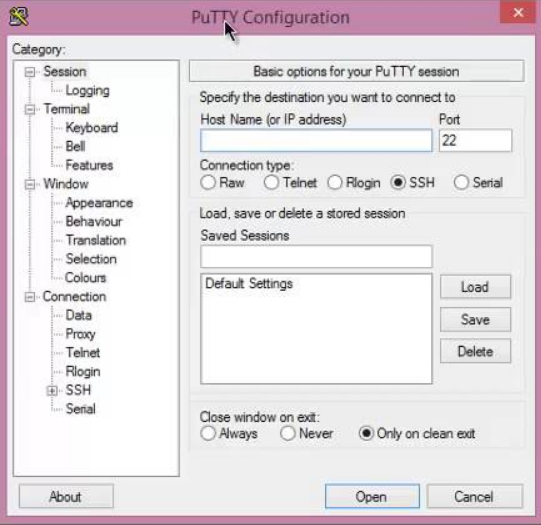
\includegraphics[scale=0.5]{putty_config}

For the port, use 22; for the connection type, use SSH. For the host name, use \lstinline{pcXX.cs.ucdavis.edu}, where \lstinline{XX} is the number of the computer that you wish to log into. Click Open. It should at some point ask for your username and password, at which point you enter your Kerberos username and password (the ones that you use to log in to Schedule Builder).

\textbf{Transferring files to/from the CSIF}: As you will submit your assignment on Gradescope, you will need to transfer your files from the CSIF to your computer. You can do this with the \lstinline{scp} command. The \lstinline{scp} command behaves the same as the \lstinline{cp} command, except that either the source or the destination is on a remote host. Below is an example in which I transfer a file to the CSIF, log on to the CSIF to modify it, and then transfer the file back to my computer.

\begin{lstlisting}
$ echo "Blah" > foo.txt
$ cat foo.txt 
Blah
$ scp foo.txt aaron123@pc43.cs.ucdavis.edu:~/tmp/foo.txt
aaron123@pc43.cs.ucdavis.edu's password: 
foo.txt                                                            100%    5     0.2KB/s   00:00    
$ ssh aaron123@pc43.cs.ucdavis.edu
aaron123@pc43.cs.ucdavis.edu's password: 

*
* Computer Science Instructional Facility
* Ubuntu 18.04.5 LTS
*
...
aaron123@ad3.ucdavis.edu@pc43:~$ cat tmp/foo.txt 
Blah
aaron123@ad3.ucdavis.edu@pc43:~$ echo "changing the contents" > tmp/foo.txt 
aaron123@ad3.ucdavis.edu@pc43:~$ cat tmp/foo.txt 
changing the contents
aaron123@ad3.ucdavis.edu@pc43:~$ exit
logout
Connection to pc43.cs.ucdavis.edu closed.
$ scp aaron123@pc43.cs.ucdavis.edu:~/tmp/foo.txt blah.txt
aaron123@pc43.cs.ucdavis.edu's password: 
foo.txt                                                            100%   22     1.1KB/s   00:00    
$ cat blah.txt 
changing the contents
$ 
\end{lstlisting}

If you are a Windows user, you can use WinSCP to transfer files with a GUI. If you are a Mac user, I think there is a similar program called Cyberduck. I don't know if there is an equivalent for Linux users, but then again, if you have a Linux computer and are trying to avoid using the command line, I question why you bought a Linux computer in the first place :)

\textcolor{red}{Update regarding file line endings}: If you transfer a file from a Windows machine to the CSIF, you may run into issues involving the fact that file line endings are different on a Windows machine vs. a Linux machine. You can use the \lstinline{dos2unix} command to get around this. Specifically, once you have your file transferred onto the CSIF, you can run \lstinline{dos2unix} on it, and that will change the line endings.

\textbf{If you use the CSIF from a different time zone}, be wary of this message on the \href{http://csifdocs.cs.ucdavis.edu/home}{front page of the CSIF website}: ``Please note that the computers restart once each day between the hours of 3:30 a.m. to 4:00 a.m. and updates will run from 4:30 a.m. to 6:00 a.m. every day.''

\end{document}